\documentclass{slide}

\usepackage{changepage}
\usepackage{tabto}
% \usepackage{pgfpages}

% \setbeameroption{show notes on second screen}

\title{Service-Based Architecture}
\subtitle{CSSE6400}
\author{Richard Thomas}
\date{\week{4}}

\begin{document}

\maketitle

\definition{Distributed System}{A system with multiple components located on different machines that communicate and coordinate actions in order to appear as a single coherent system to the end-user.}
\note{Introduce idea of distributed systems and then move on to service-based being an simple approach.}

\point[Quote]{A distributed system is one in which the failure of a computer you didn't even know existed can render your own computer unusable.\\
 ~~~~~ -- Leslie Lamport [Turing Award, 2013]}

\definition{Service-Based Architecture}{System is partitioned into business domains that are deployed as distributed services.
Functionality is delivered through a user interface that interacts with the domain services.}
\note{Explain why this leads to a fairly simple distributed architecture.}

\begin{frame}{Service-Based Architecture}
    \begin{adjustwidth}{-10mm}{-10mm}
        \centering
        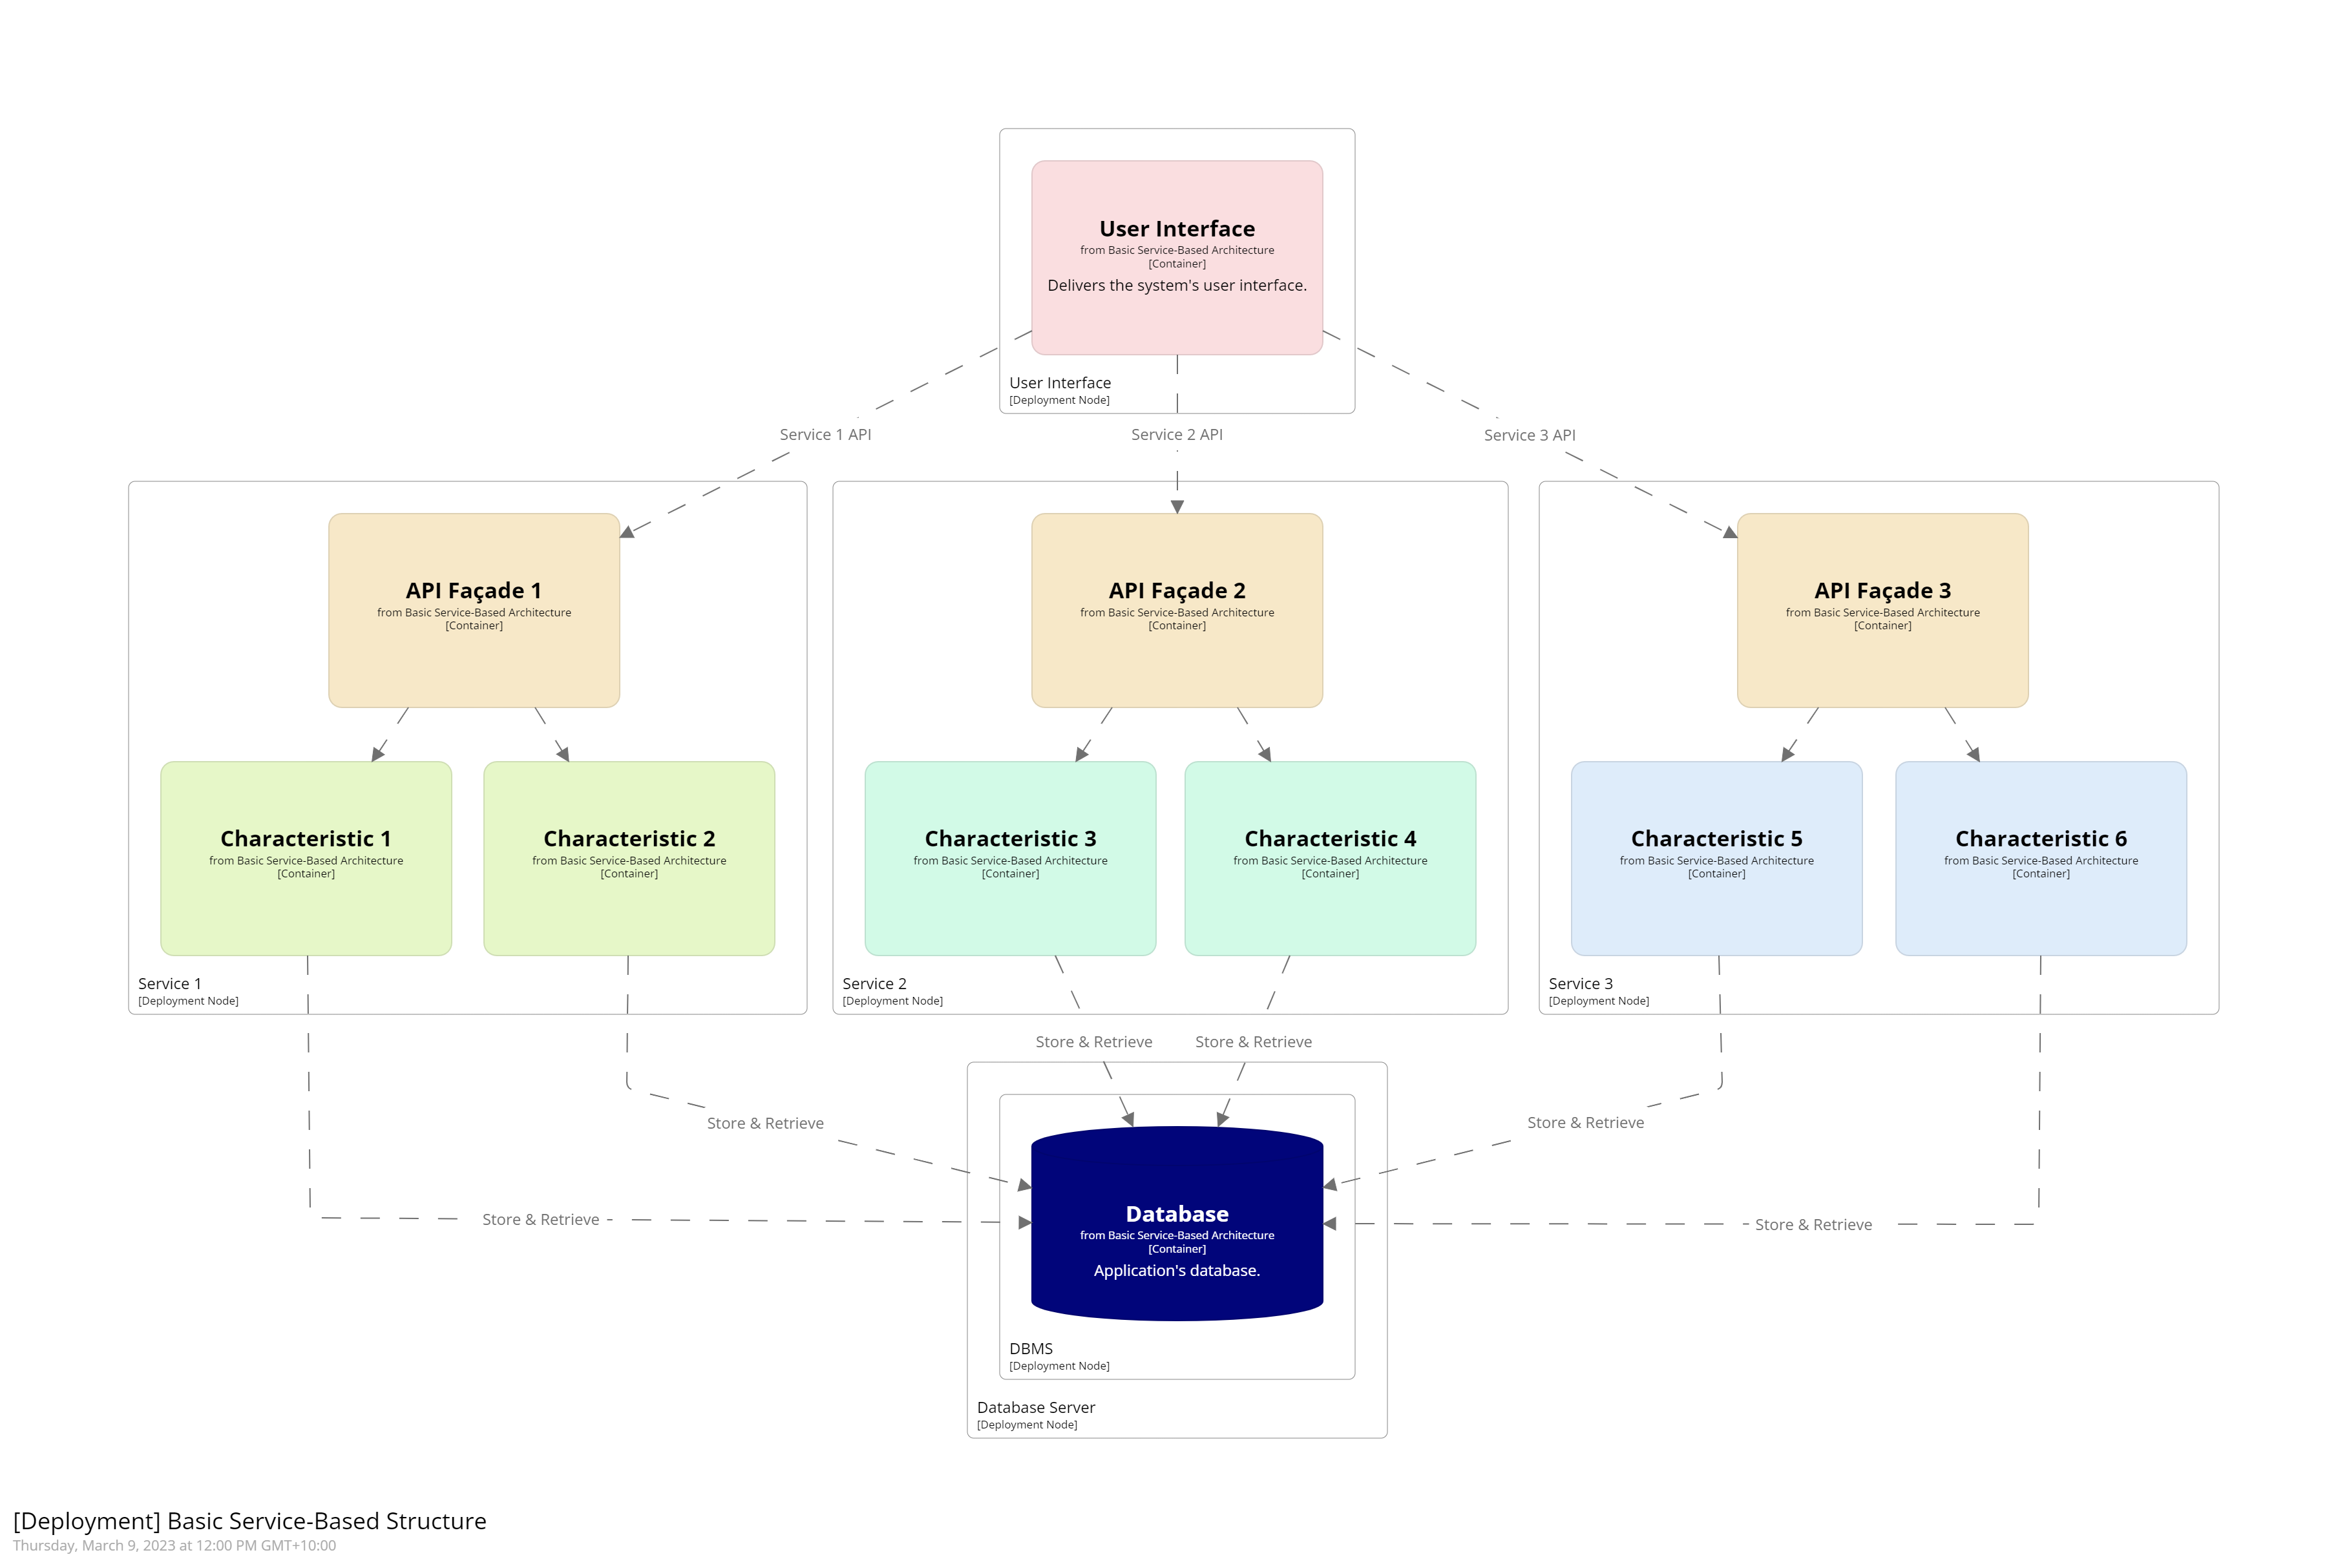
\includegraphics[trim=39 43 19 44,clip,width=0.97\paperwidth]{../../notes/service-based/diagrams/general-service-based-arch.png}
    \end{adjustwidth}
\end{frame}

\begin{frame}{Terminology}
    \vspace{1mm}
    {\LARGE
    \begin{description}
        \item[User Interface] Provides access to system functionality
        \vspace{3mm}
        \item[Services] Implement functionality for a single, independent business process
        \vspace{3mm}
        \item[Service APIs] Communication mechanism between UI and each service
        \vspace{3mm}
        \item[Database] Stores persistent data for the system
    \end{description}
    }
\end{frame}
\note[itemize]{
    \item Explain that the Service APIs are communication protocols and data formats, not just a Java-style interface.
    \item Usually all Service APIs use the same communication protocol (e.g. REST).
    \item Also point out that messages between the UI and services will typically be asynchronous.
}

\definition{API Abstraction Principle}{Services should provide an API that hides implementation details.}
\note[itemize]{
    \item Each service publishes its own API.
    \item Hides service implementation details, reducing coupling between UI and service.
    \item Makes it easier to reuse service across systems or by supporting service (e.g. auditing).
}

\definition{Façade Design Pattern}{Provide a simple, abstract interface to use a service domain's functionality.
A component within the service coordinates how to deliver the requested functionality with the service's internal components.}
\note{Summarise Façade Design Pattern and how it is used in a service-based architecture. Mention its from the GoF book.}

\definition{Independent Service Principle}{Services should be independent, with no dependencies on other services.}
\note[itemize]{
    \item Explain consequences of dependencies between services.
    \item Services can't easily be deployed separately if they depend on other services.
    \item They would require interfaces between services, increasing coupling.
}

\questionanswer{What are the consequences of having a shared database?}{Increased \highlight{data coupling}.}
\note[itemize]{
    \item If a row of a database is locked and another service wants to use it, it is blocked. Losing efficiency benefits of a distributed system.
    \item If one service changes the structure of its persistent data, all services using that data need to be updated and tested.
    \item If one service changes how it uses persistent data, all other services using the same data need to be retested.
}

\begin{frame}{Logical Partitioning of Persistent Data}
    \centering
    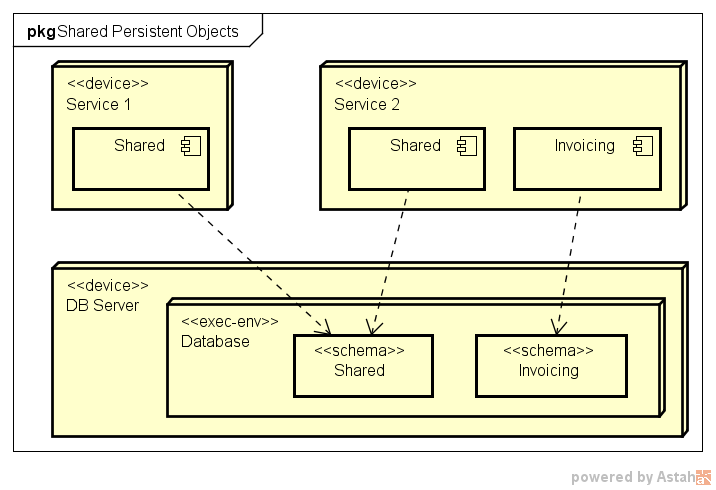
\includegraphics[trim=37 37 20 44,clip,width=0.8\textwidth]{../../notes/service-based/diagrams/db-logical-partitioning.png}
\end{frame}
\note[itemize]{
    \item Define a minimal set of shared persistent objects.
    \item Create a shared library to access these objects.
    \item Changes to shared persistent objects are restricted as they require changes to other services.
    \item Each service may have its own persistent objects stored in tables that are not shared with other services.
}

\begin{frame}{Separate Databases}
    \centering
    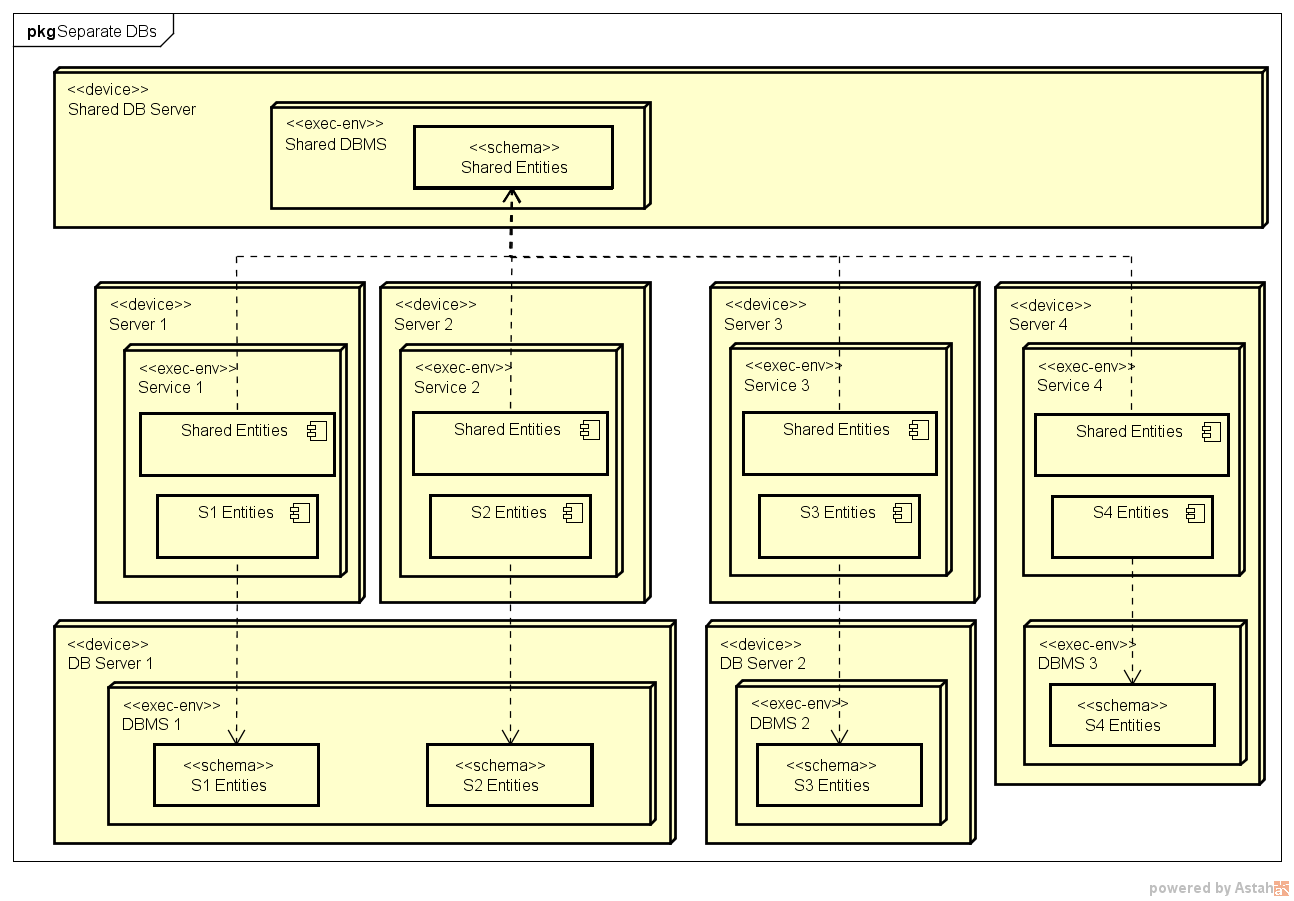
\includegraphics[trim=39 42 18 48,clip,width=0.9\textwidth]{../../notes/service-based/diagrams/separate-dbs.png}
\end{frame}
\note{Discuss options of separate DB servers, share DBs on one server, DBs embedded in application.}

\begin{frame}{Separate UIs}
    \centering
    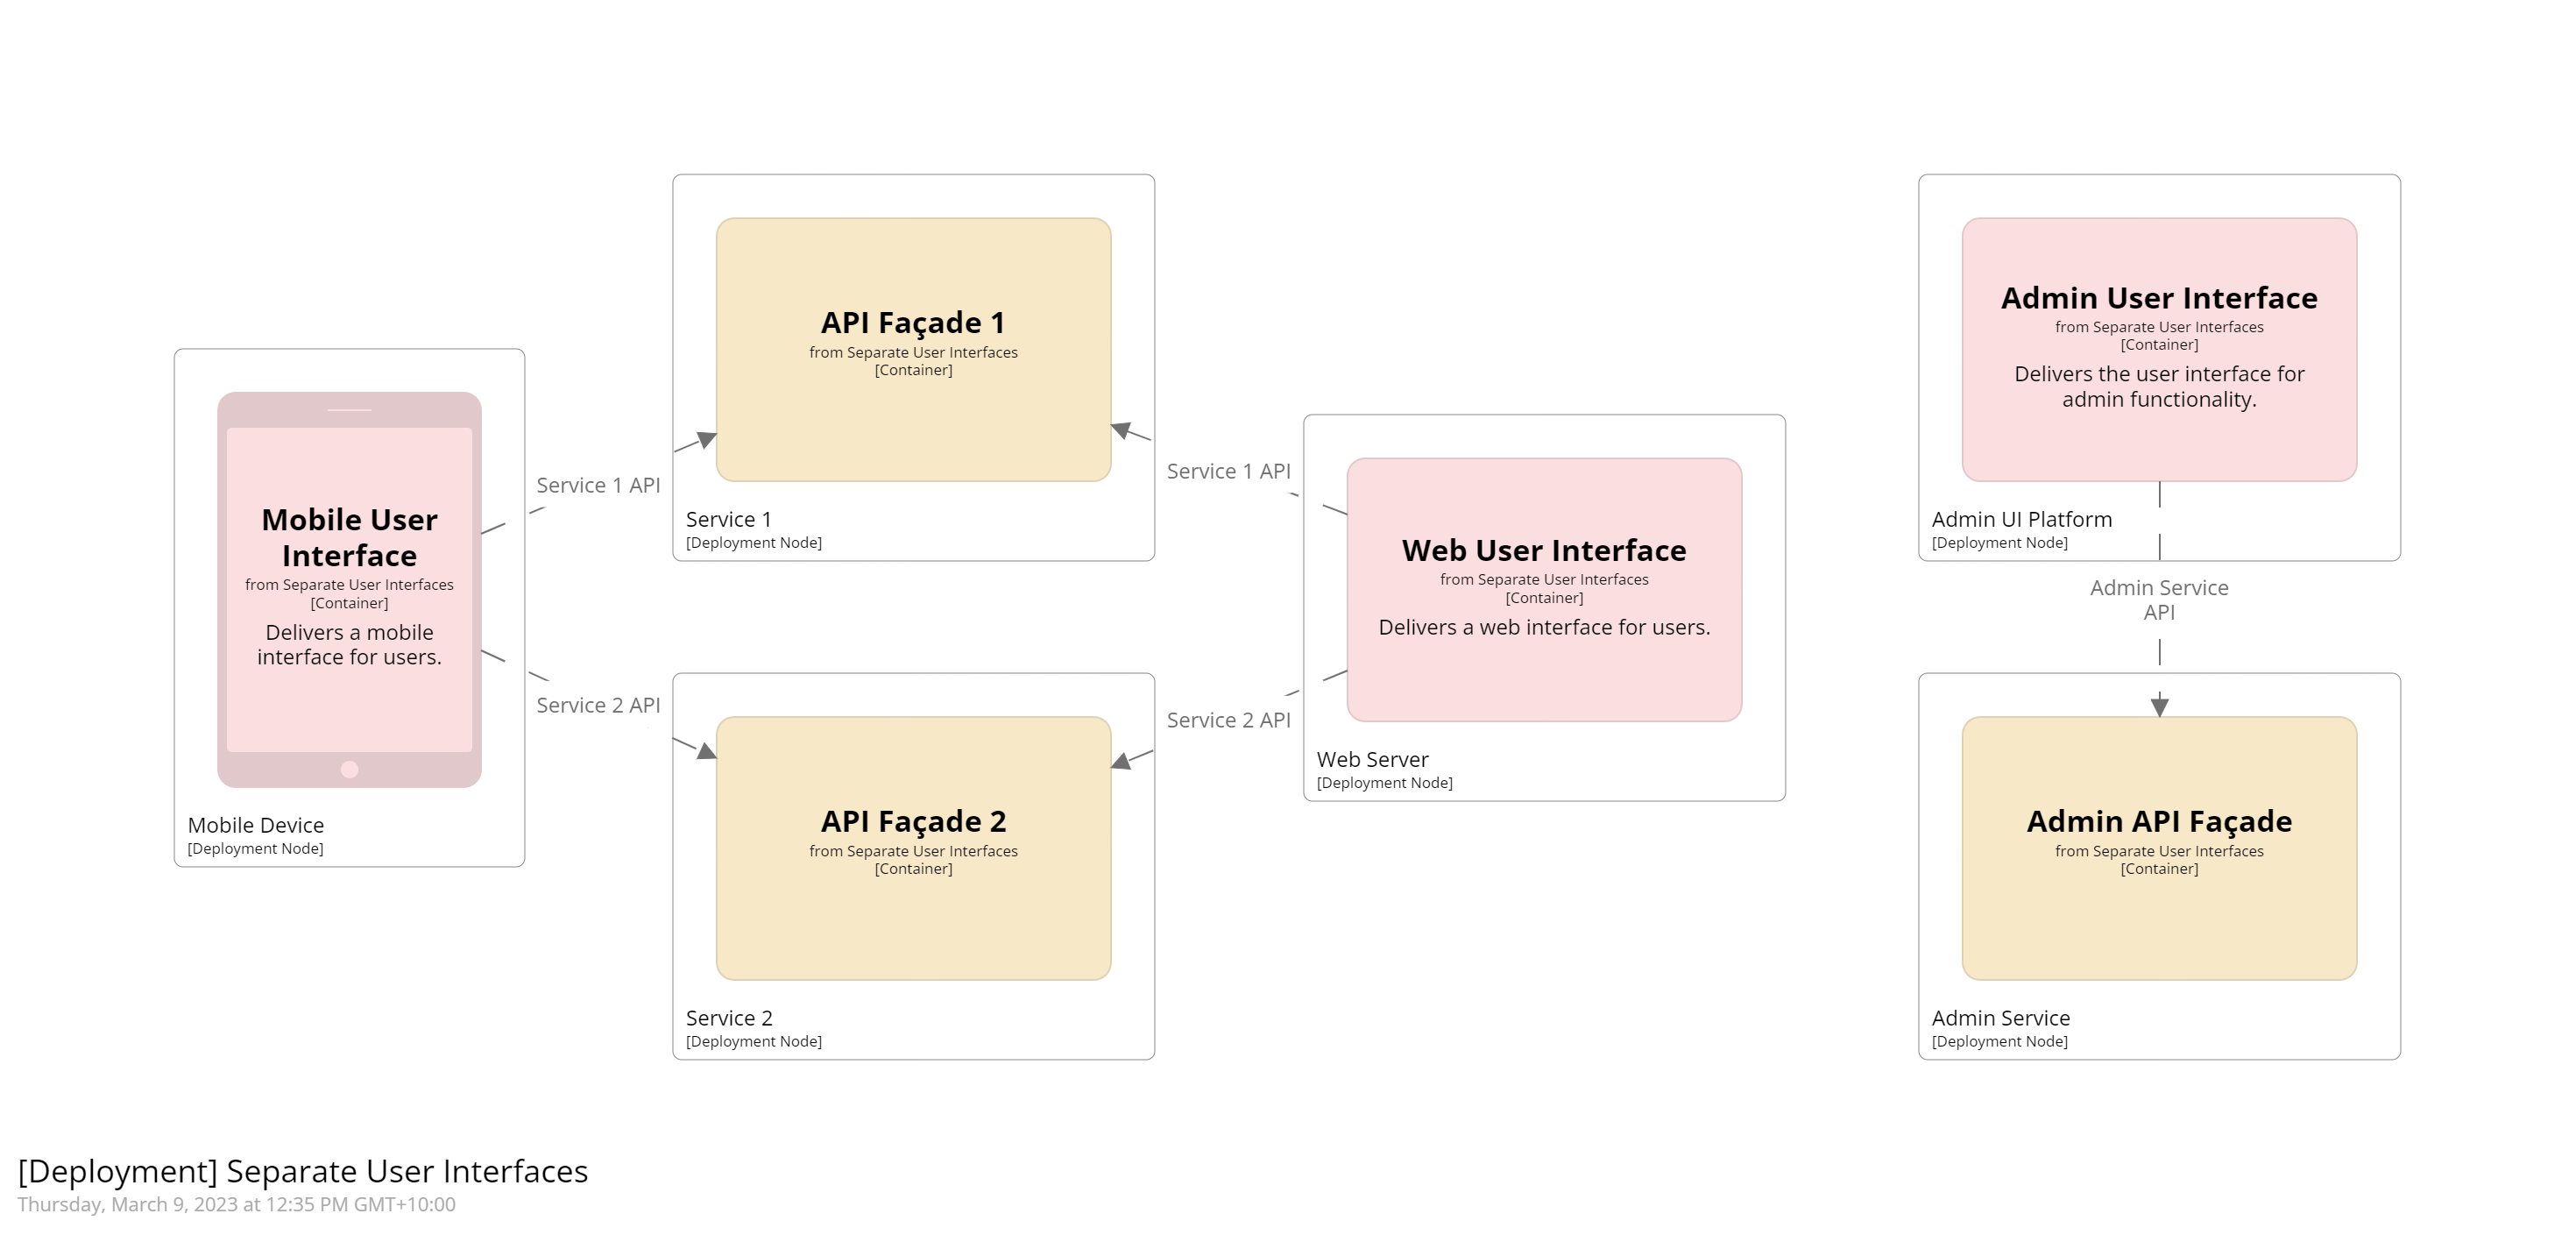
\includegraphics[trim=40 42 19 45,clip,width=\textwidth]{../../notes/service-based/diagrams/separate-uis.png}
\end{frame}
\note[itemize]{
    \item UI Platform could be desktop, web or mobile app.
    \item This allows multiple concurrent users, even through one user interface.
}

\begin{frame}{Sahara: Context Diagram}
    \centering
    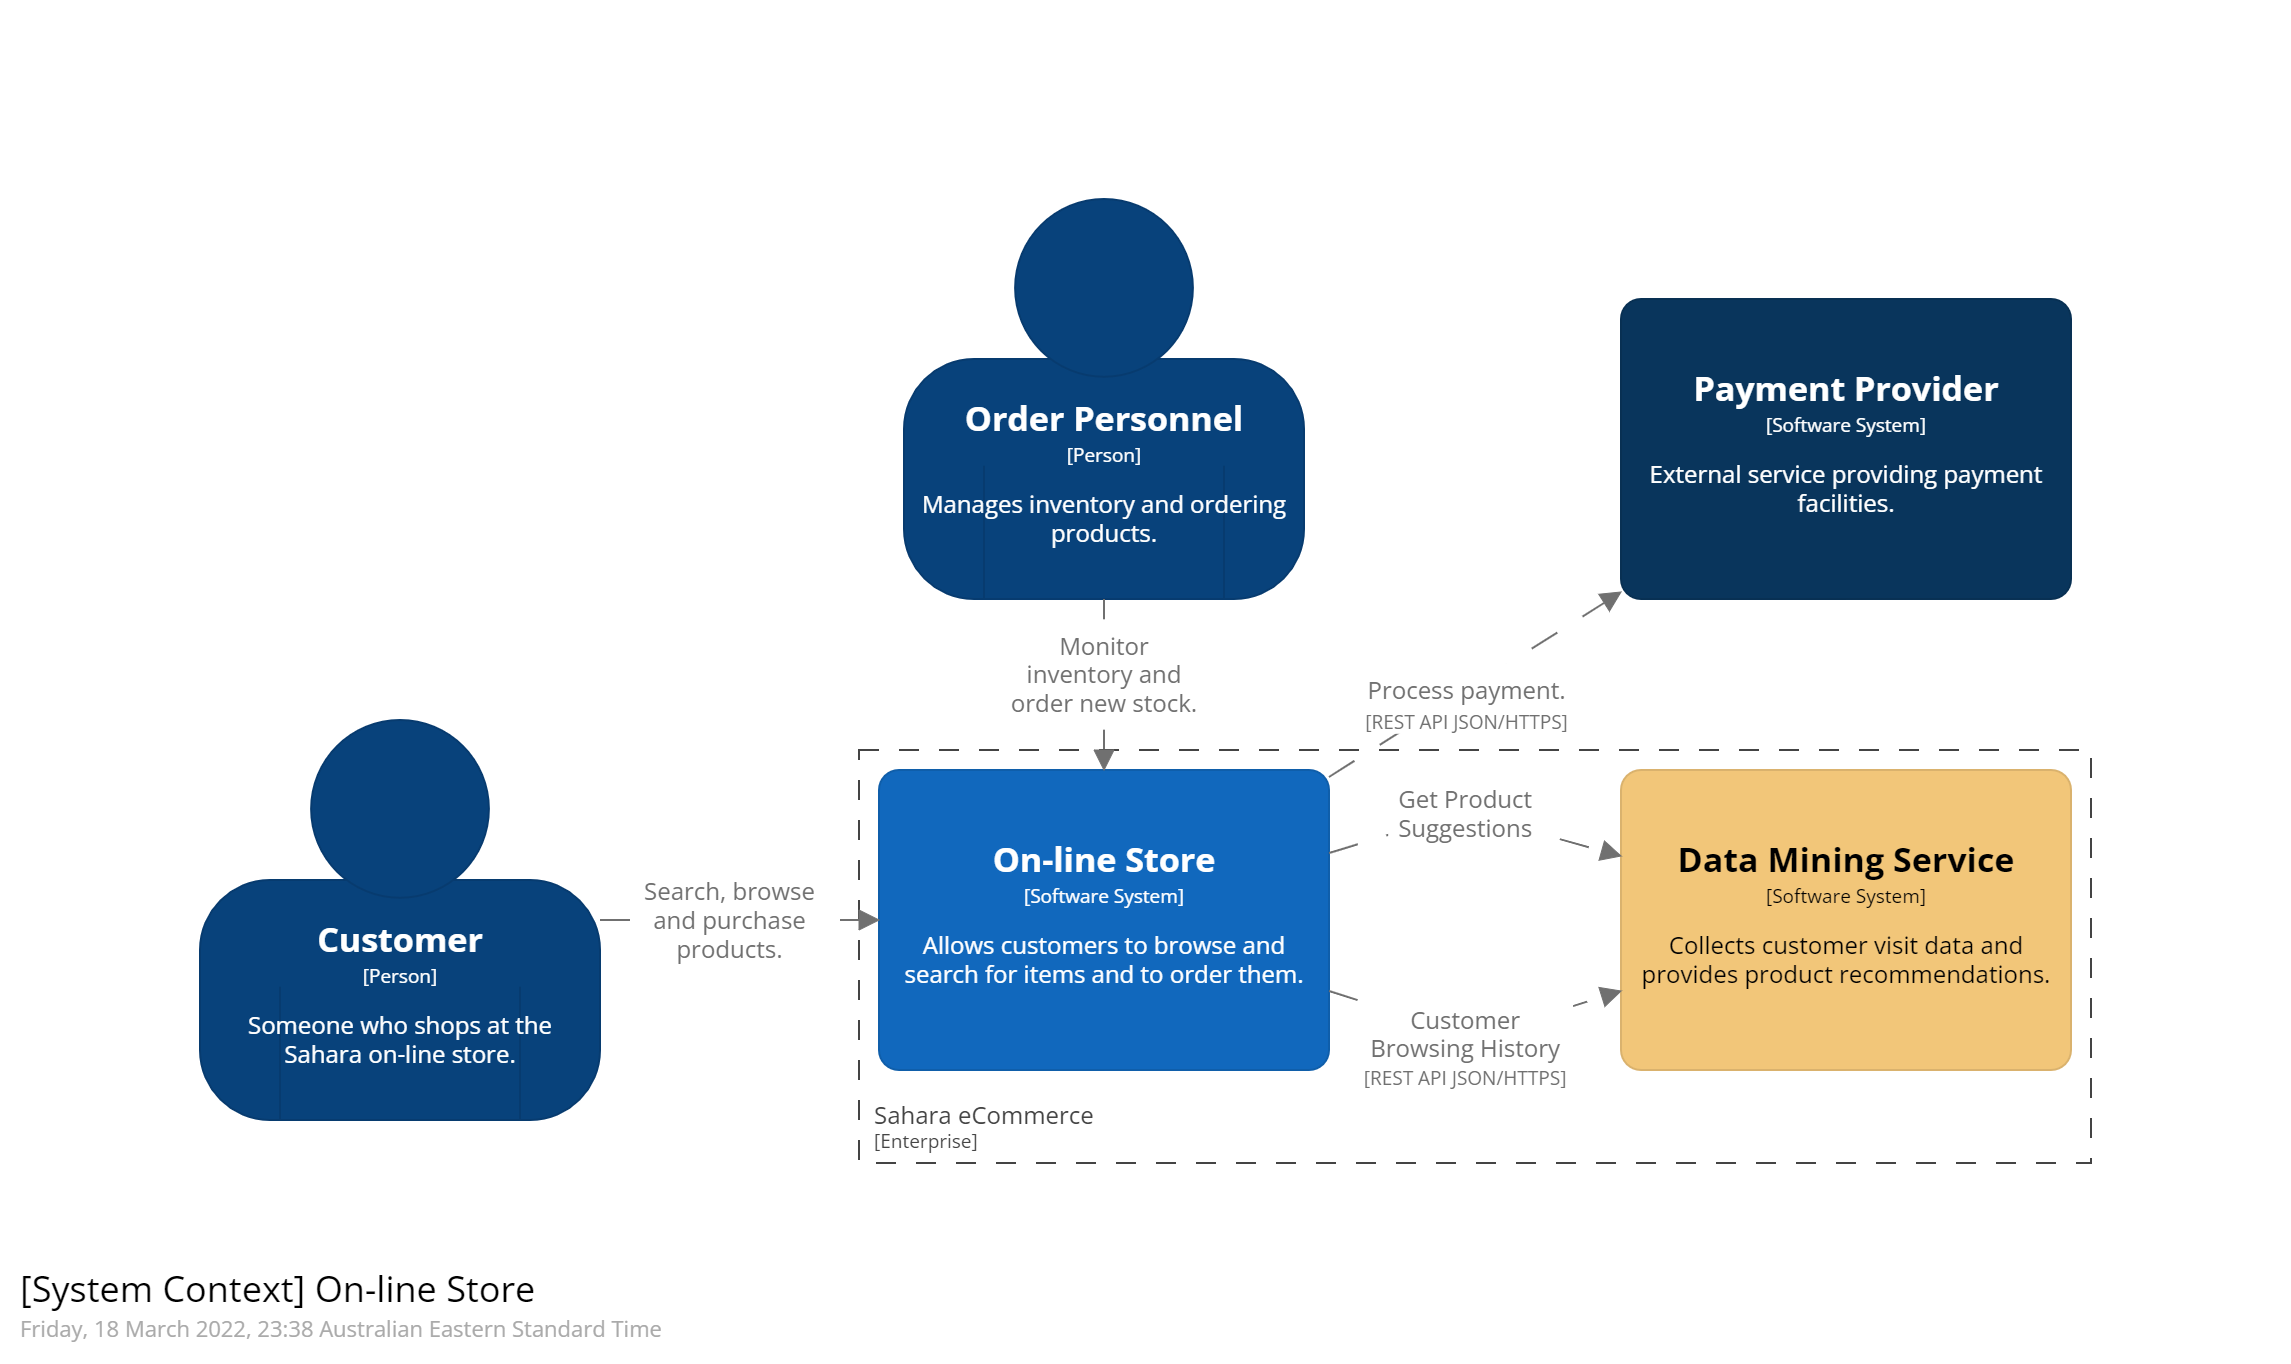
\includegraphics[trim=195 195 195 195,clip,width=\textwidth]{diagrams/sahara-context.png}
\end{frame}
\note[itemize]{
    \item Summarise Sahara eCommerce example.
    \item Order Personnel \& Payment Provider added to this example.
}

\begin{frame}{On-line Store Service Domains}
    \vspace{1mm}
    {\LARGE
    \begin{description}
        \item[Browsing] Customers can find products \& add to cart
        \item[Purchasing] Customers can purchase products in cart
        \item[Fulfilment] Customers \& staff can track order fulfilment
        \item[Account Management] Customers can manage their account details
        \item[Inventory Management] Staff can view stock levels and order new stock
    \end{description}
    }
\end{frame}
\note[itemize]{
    \item Mention that service-based architectures are based on domain partitioning.
    \item Could provide examples of fulfilment, and inventory management activities.
    \item Customer's tracking order, staff generating pick lists and packaging details.
    \item Generating reports on stock levels and product popularity. Ordering new stock.
}

\point[Partitioning]{Services are defined by domain partitioning}

\begin{frame}{Coarse Services}
    \vspace{1mm}
    {\LARGE
    \begin{itemize}
        \item Domains are large
        \begin{itemize}
            \Large\item \highlight{Coarse-grained} services
        \end{itemize}
        \vspace{2mm}
        \item Each service will have an internal architecture
        \begin{itemize}
            \Large\item Technical or domain partitioning
        \end{itemize}
    \end{itemize}
    }
\end{frame}

\begin{frame}{Sahara: On-line Store Container Diagram}
    \begin{adjustwidth}{-5mm}{-5mm}
        \centering
        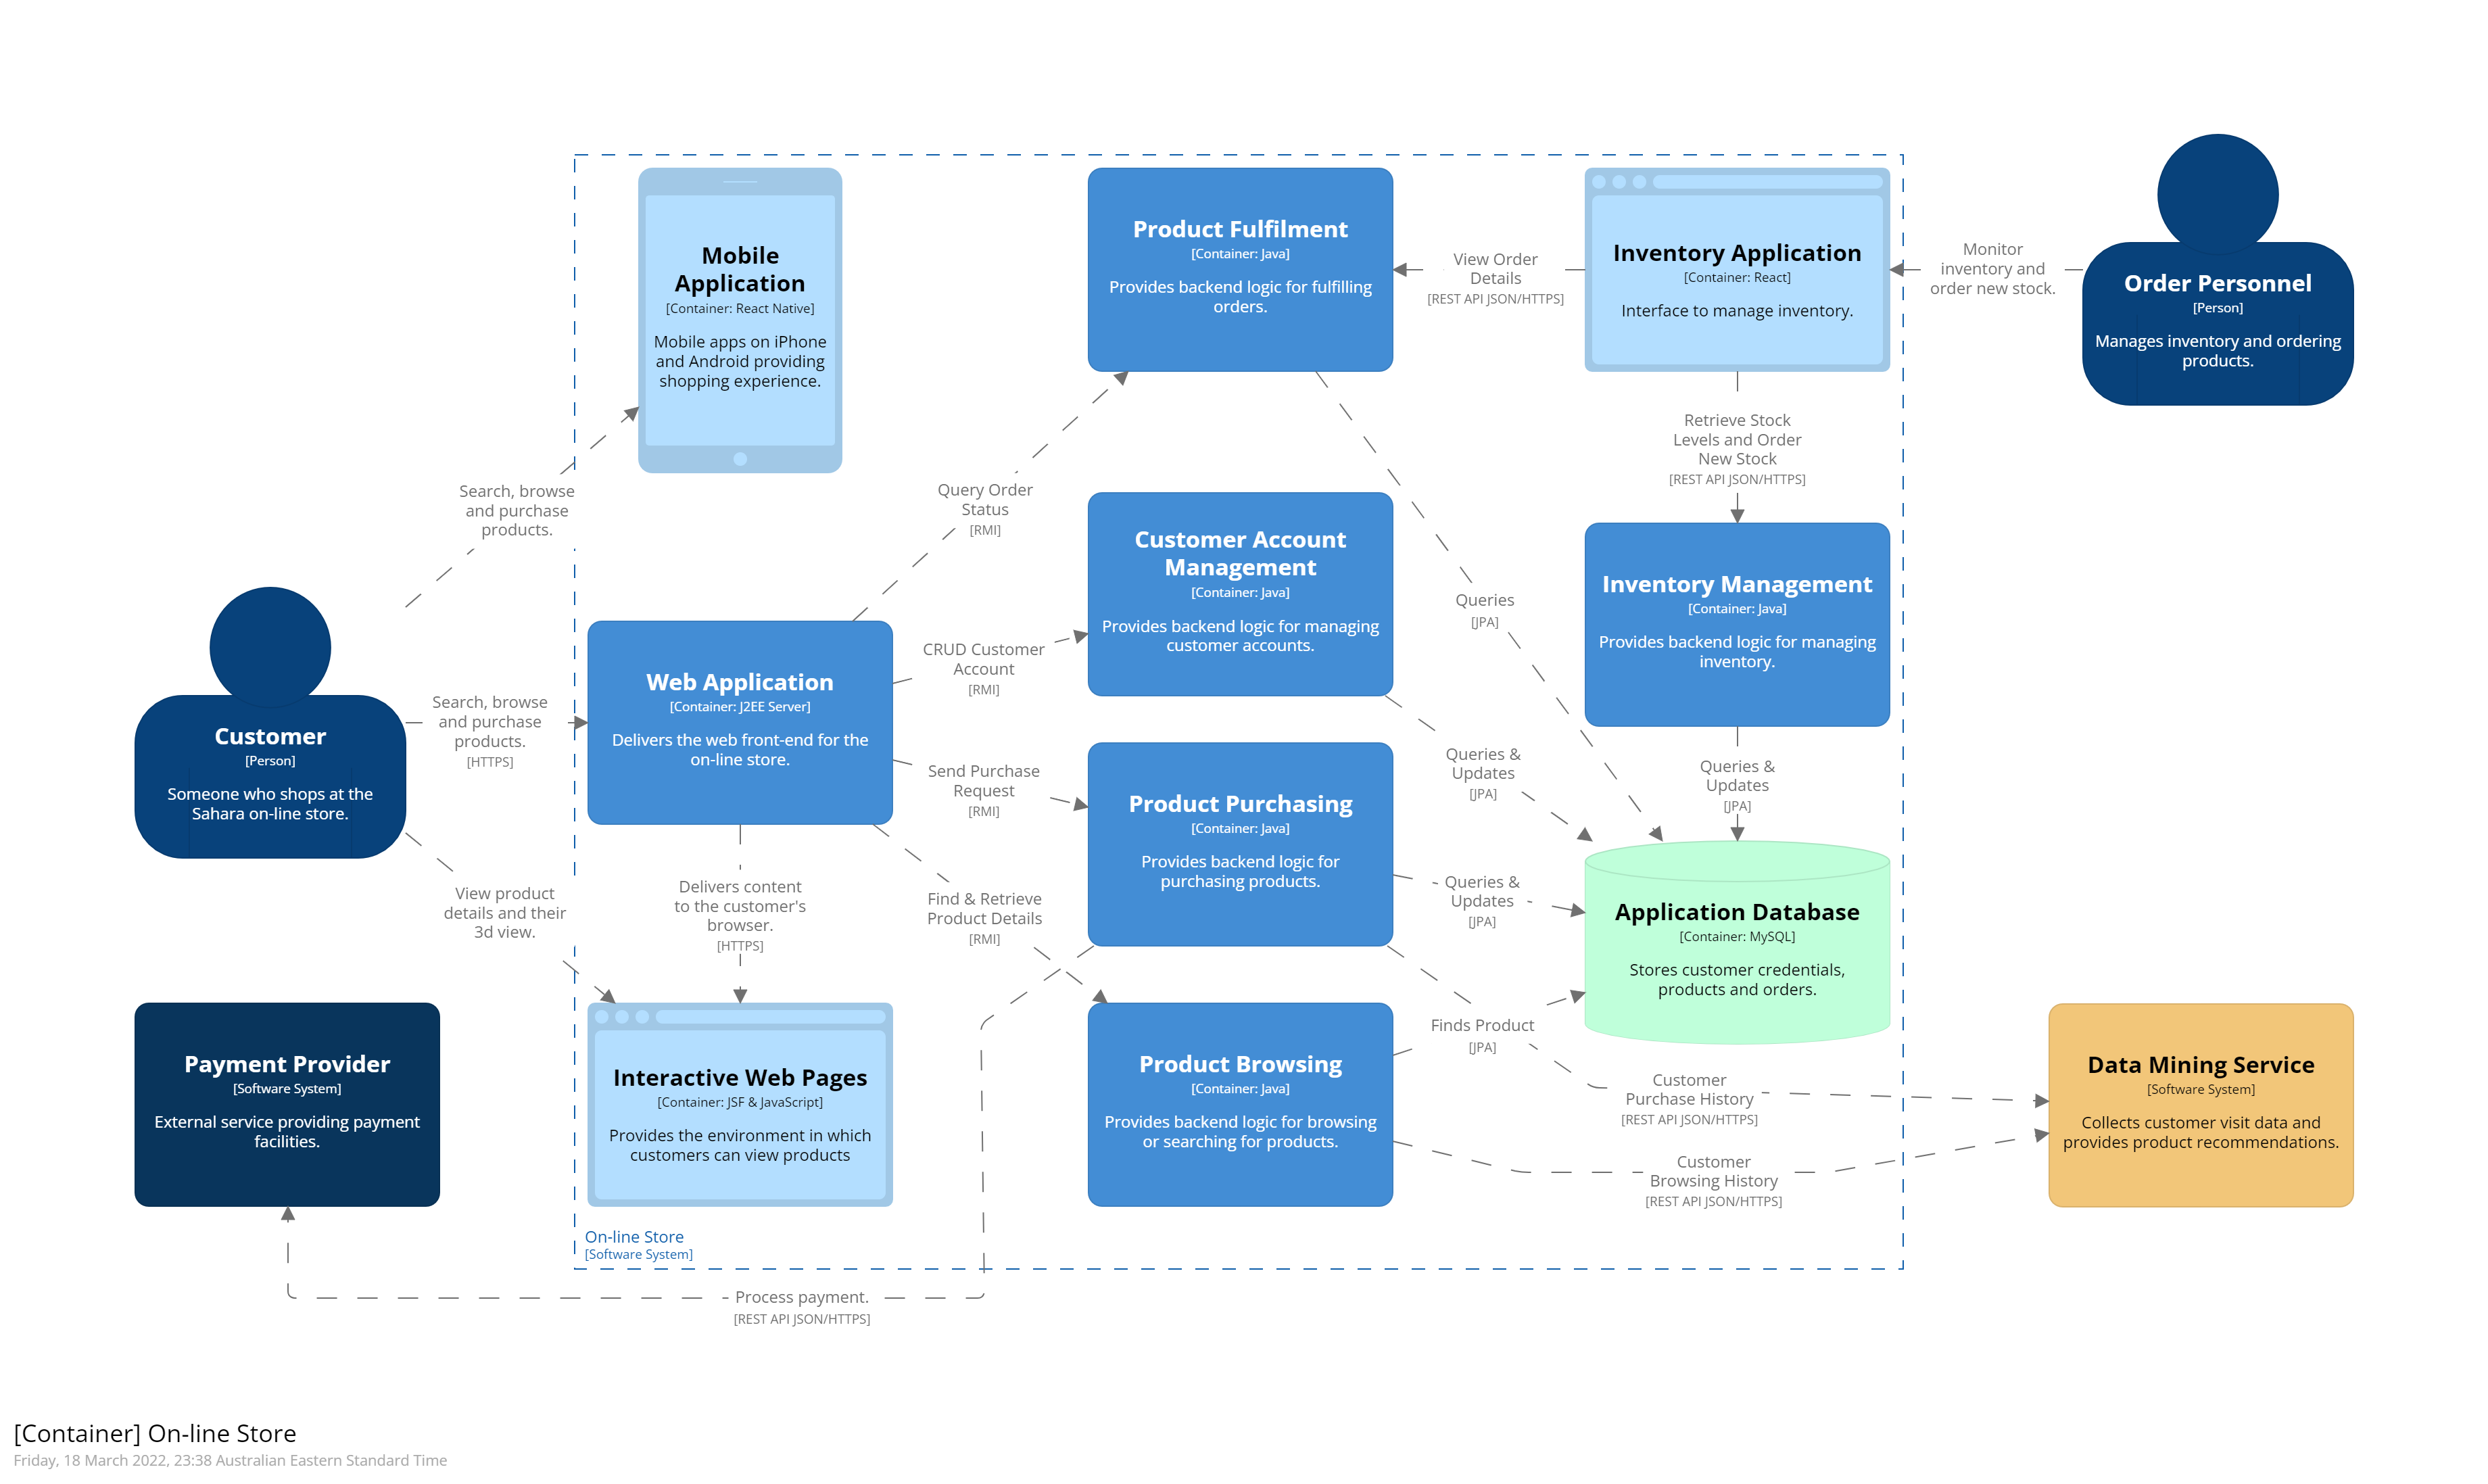
\includegraphics[trim=190 230 190 190,clip,width=0.935\paperwidth]{diagrams/sahara-container-store.png}
    \end{adjustwidth}
\end{frame}
\note[itemize]{
    \item Review Domain Services in context of the overall system.
    \item Mobile App relationships not shown to reduce clutter.
    \item Single DB for simplicity of diagram, not good practice. Should be split.
    \item Cart needs to be shared with Browsing \& Purchasing.
    \item Order needs to be shared with Purchasing \& Fulfilment.
    \item Product needs to be shared with everything except Account Management.
    \item User needs to be shared with almost everything.
    \item Most of these will be query only, or only locking a single row of some tables.
    \item Repeat idea that Service APIs mean you may have multiple UIs (Web, Mobile, Inventory Apps).
}

\begin{frame}{Sahara: Product Browsing Component Diagram}
    \begin{adjustwidth}{-10mm}{-10mm}
        \centering
        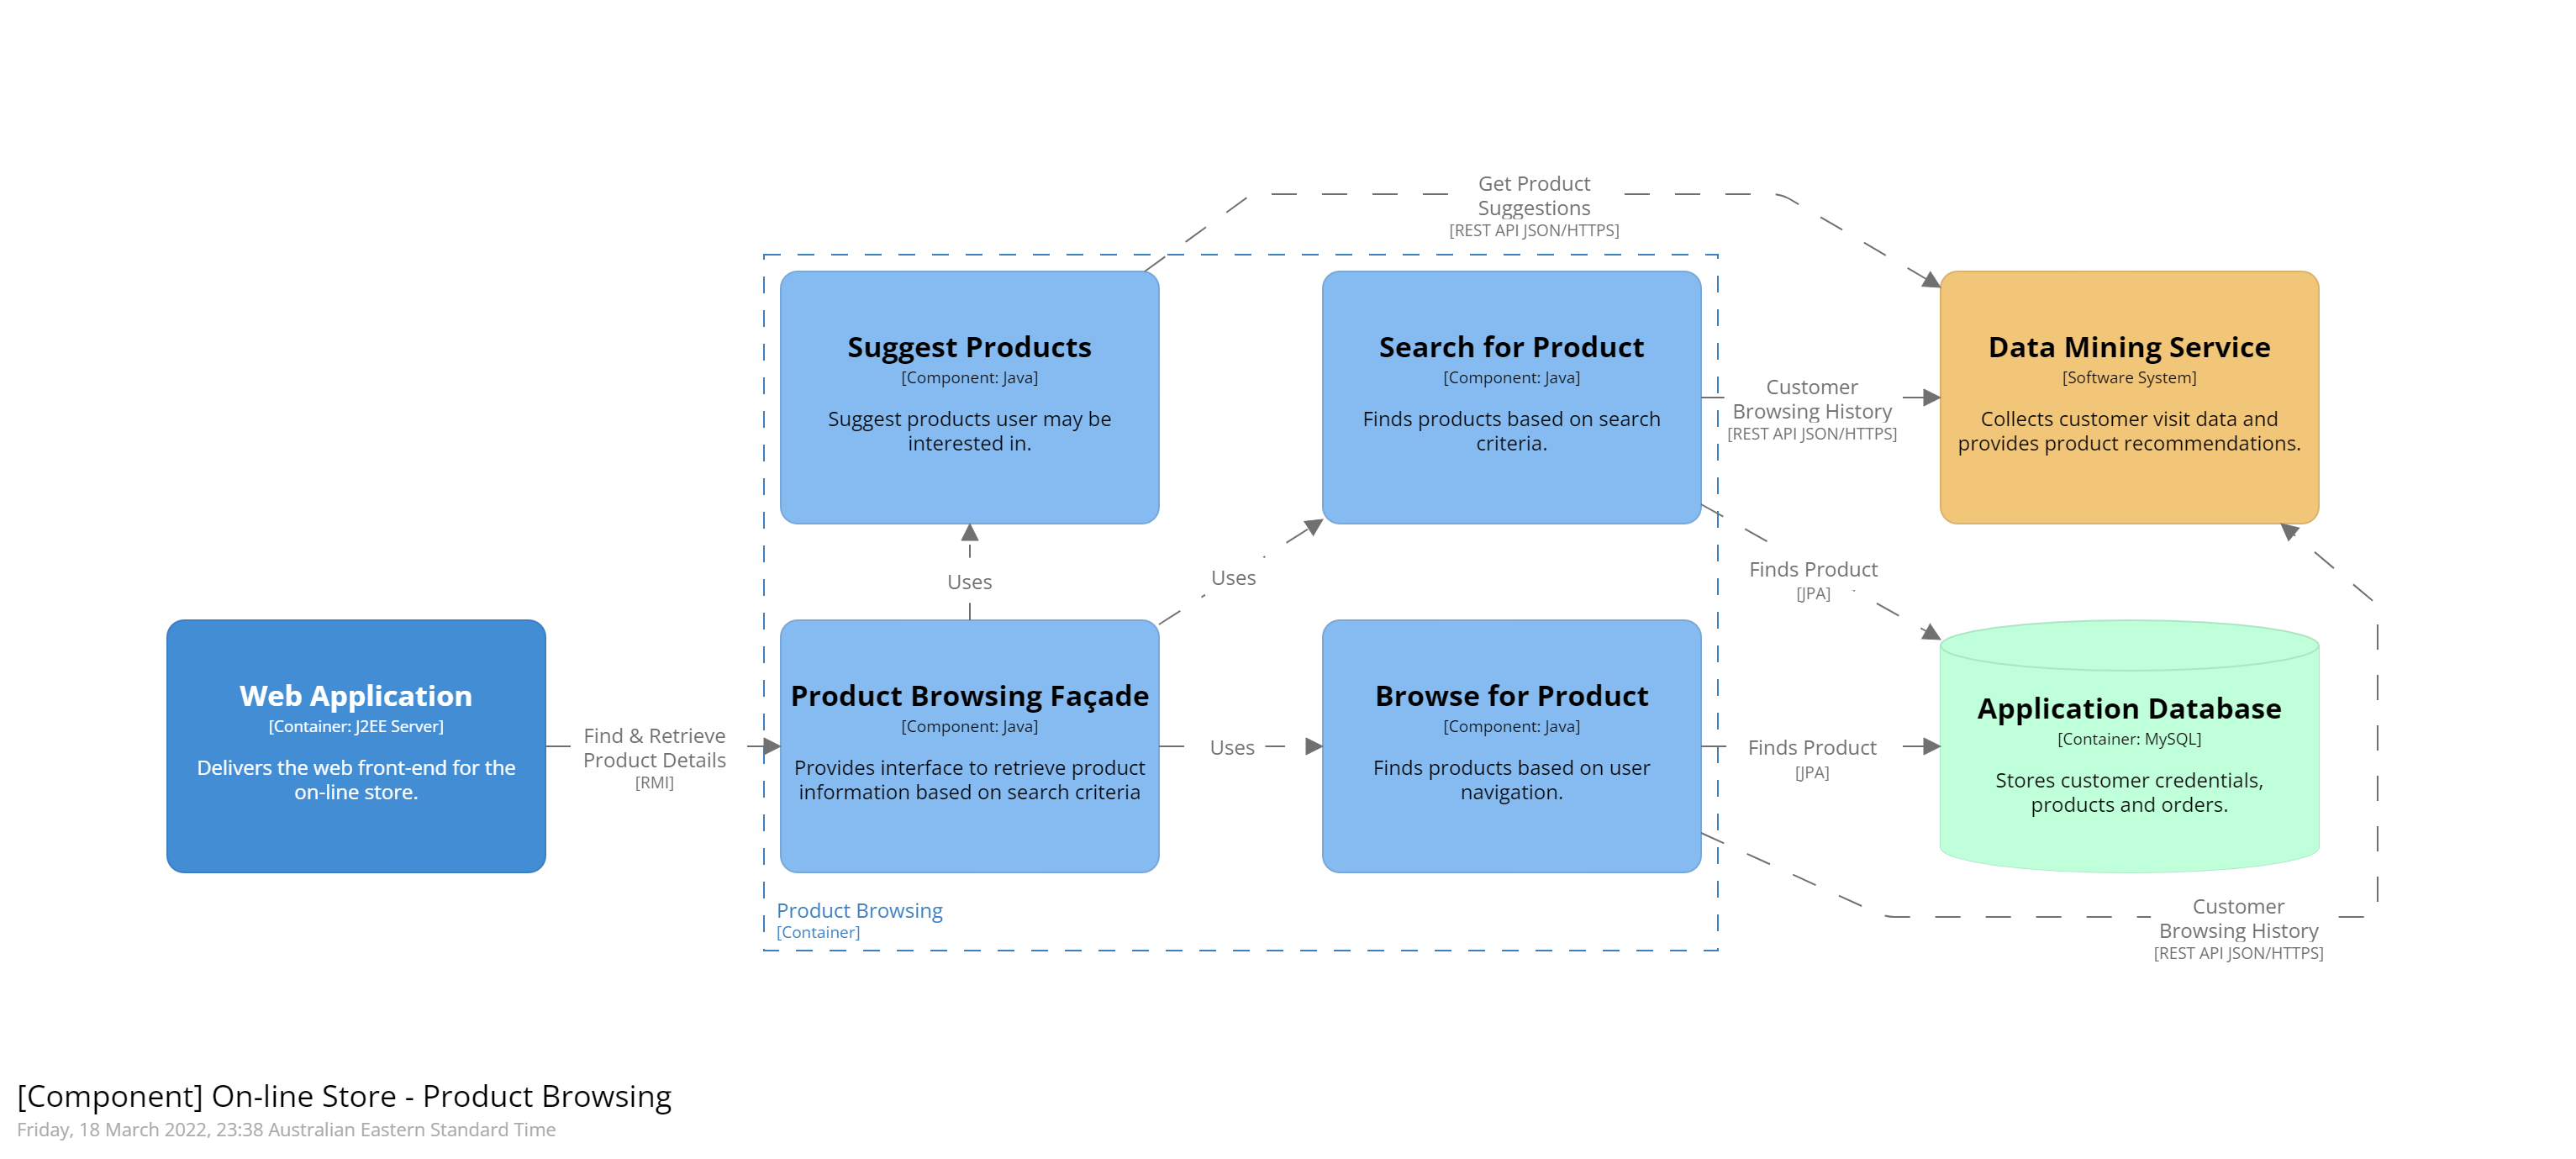
\includegraphics[trim=190 200 230 200,clip,width=0.97\paperwidth]{diagrams/sahara-component-browse.png}
    \end{adjustwidth}
\end{frame}
\note[itemize]{
    \item Summarise the components making up the key parts of the Product Browsing Service (container).
    \item Product Browsing Façade provides the Service API.
}

\begin{frame}{Product Browsing Service API}
    \vspace{1mm}
    {\LARGE
    \begin{description}
        \item[Search] https://api.sahara.com/v1/search?keywords=...
        \item[Browse] https://api.sahara.com/v1/browse?category=...
        \item[Add to Cart] https://api.sahara.com/v1/cart
    \end{description}
    \vspace{4mm}
    \begin{itemize}
        \item JSON to pass data
        \item JSF action controller handles request
    \end{itemize}
    }
\end{frame}
\note[itemize]{
    \item Search \& Browse are GET requests passing parameters.
    \item Add to Cart is a POST request passing product id and quantity to be added to cart.
    \item Authentication needs to be part of requests.
    \item API Versioning shown in URIs.
}

\begin{frame}{Sahara: Deployment Diagram}
    \begin{adjustwidth}{-5mm}{-5mm}
        \centering
        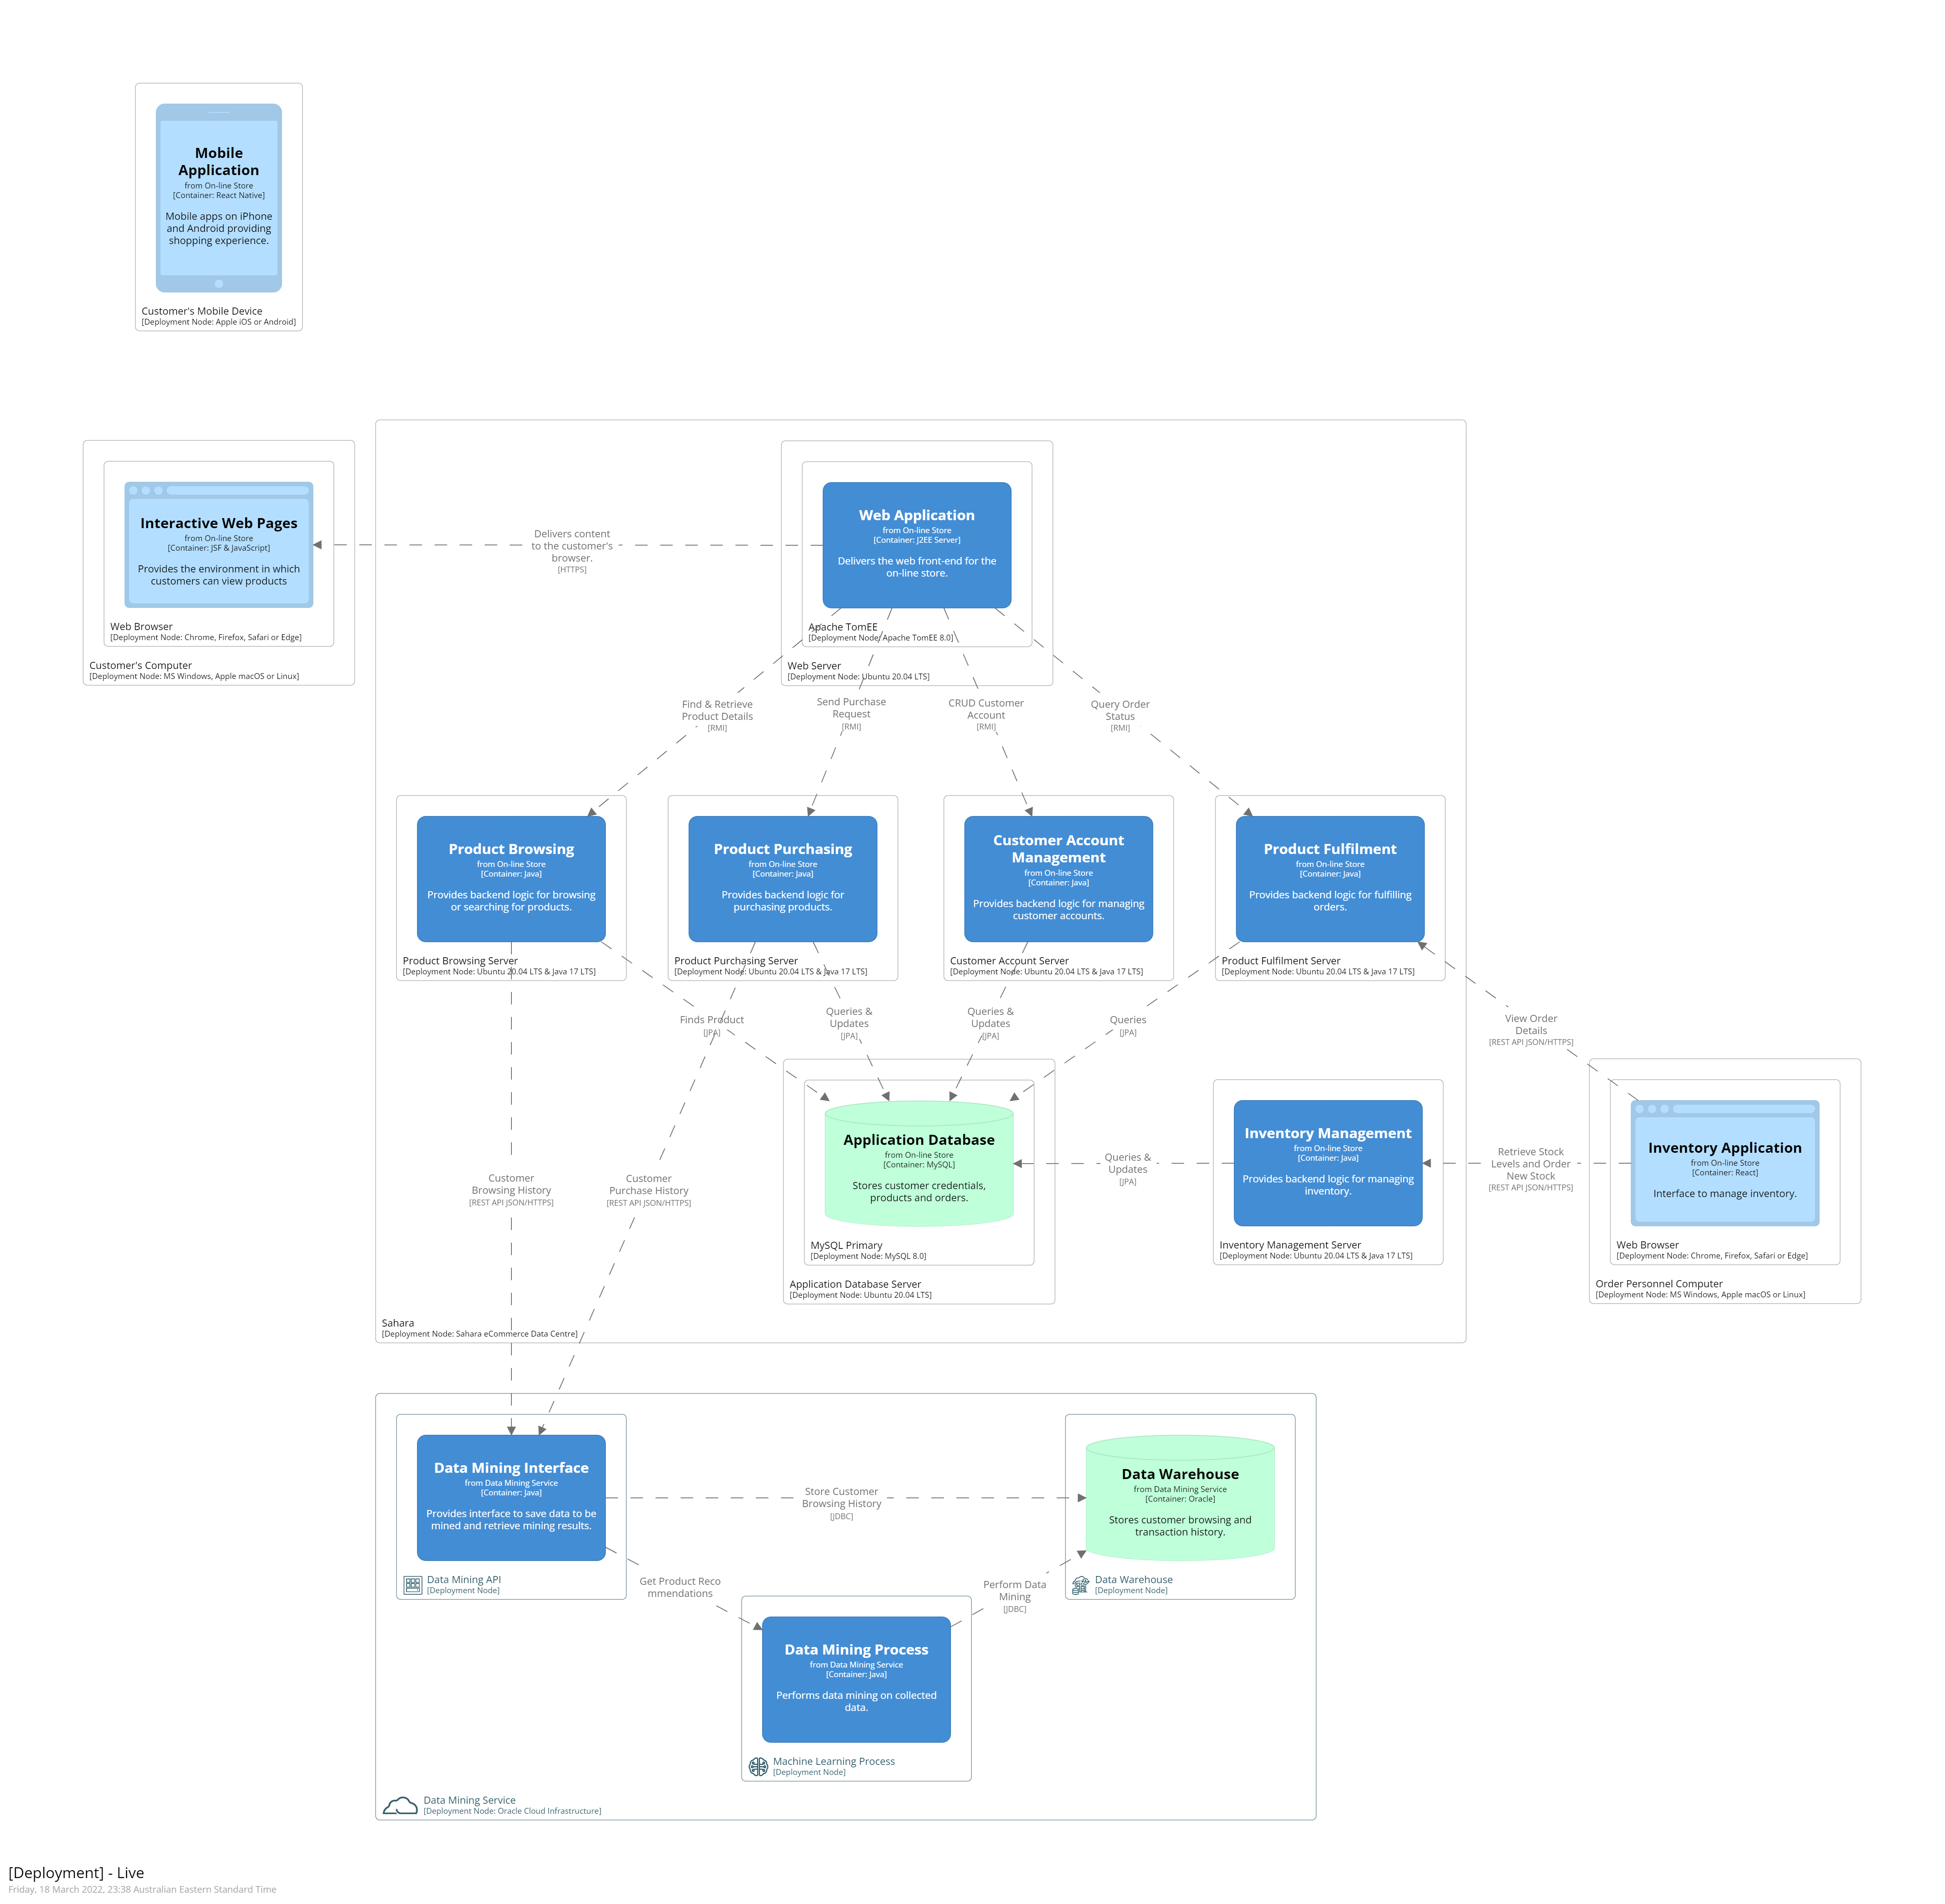
\includegraphics[trim=197 1340 197 1002,clip,width=0.935\paperwidth]{diagrams/sahara-deployment.png}
    \end{adjustwidth}
\end{frame}
\note[itemize]{
    \item UI Platform could be desktop, web or mobile app.
    \item This allows multiple concurrent users, even through one user interface.
}

\begin{frame}{Sahara: Concurrent Access}
    \begin{adjustwidth}{-5mm}{-5mm}
        \centering
        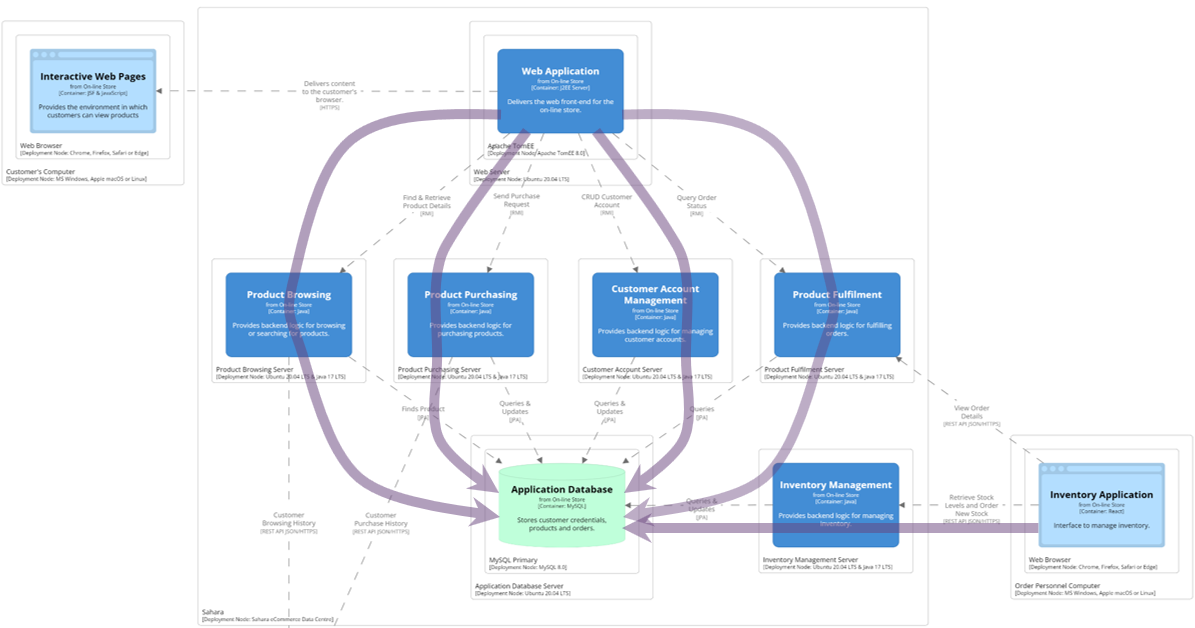
\includegraphics[trim=1 0 1 5,clip,width=0.935\paperwidth]{diagrams/sahara-concurrency.png}
    \end{adjustwidth}
\end{frame}
\note[itemize]{
    \item Emphasise many users from different UIs accessing distributed services concurrently.
    \item Point out that this \& REST require stateless services.
}

\questionanswer{What happens if a service goes down?}
{Need to manage timeouts, retries, graceful failure, \dots}
\note[itemize]{
    \item Some of this can be managed by infrastructure, which requires monitoring systems.
    \item Some issues are harder to deal with due to coarse service domains.
    \item Some of this needs to be managed within the application.
}

\begin{frame}{Consider Network Failure}
    \vspace{1mm}
    {\LARGE
    If customer tried to add product to cart:
    \begin{itemize}
        \item What happens if Product Browsing didn't receive it?
        \item What happens if UI didn't get a response?
        \item What happens if Database wasn't updated?
    \end{itemize}
    }
\end{frame}

%Failure Issues
%Failure is the defining difference between distributed and local programming, so you have to design distributed systems with the expectation of failure. Imagine asking people, "If the probability of something happening is one in 1013, how often would it happen?" Common sense would be to answer, "Never." That is an infinitely large number in human terms. But if you ask a physicist, she would say, "All the time. In a cubic foot of air, those things happen all the time."
%
%When you design distributed systems, you have to say, "Failure happens all the time." So when you design, you design for failure. It is your number one concern. What does designing for failure mean? One classic problem is partial failure. If I send a message to you and then a network failure occurs, there are two possible outcomes. One is that the message got to you, and then the network broke, and I just didn't get the response. The other is the message never got to you because the network broke before it arrived.
%
%So if I never receive a response, how do I know which of those two results happened? I cannot determine that without eventually finding you. The network has to be repaired or you have to come up, because maybe what happened was not a network failure but you died. How does this change how I design things? For one thing, it puts a multiplier on the value of simplicity. The more things I can do with you, the more things I have to think about recovering from.
% -- https://www.artima.com/articles/designing-distributed-systems

\begin{frame}{API Layer}
    \centering
    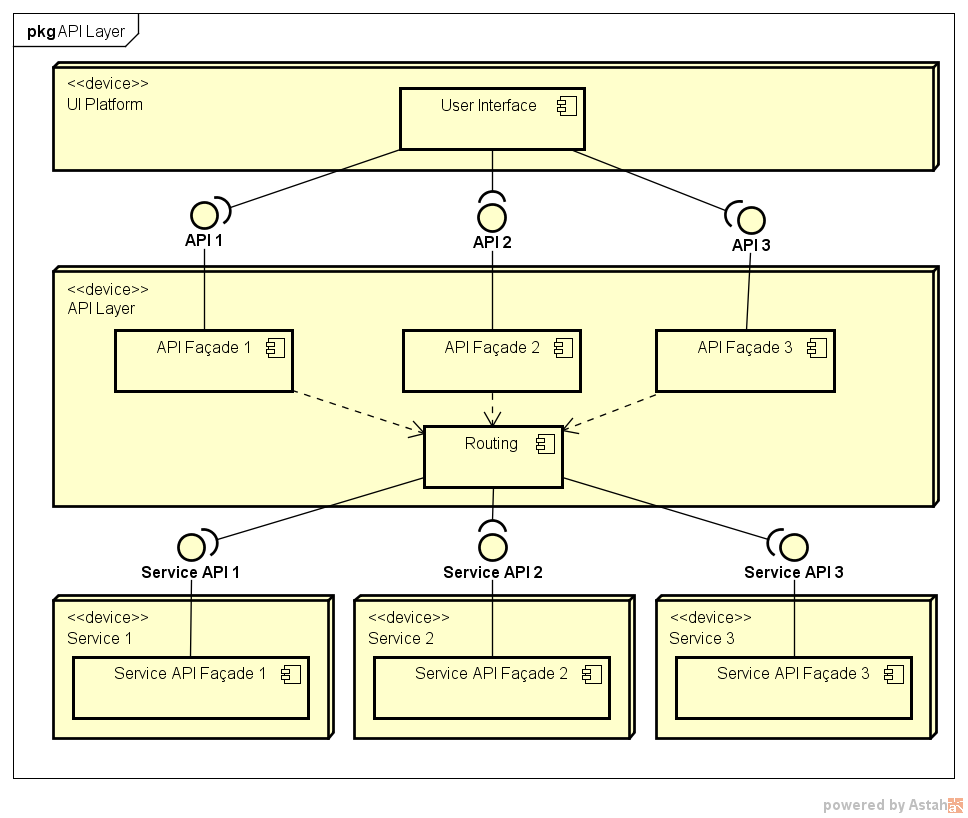
\includegraphics[trim=39 37 21 42,clip,width=0.75\textwidth]{../../notes/service-based/diagrams/api-layer.png}
\end{frame}

\begin{frame}{API Layer Advantages}
    \vspace{1mm}
    {\LARGE
    \begin{itemize}
        \item Acts as a reverse proxy or gateway to services
        \vspace{2mm}
        \item Hides internal network structure
        \vspace{4mm}
        \item Easier to implement \emph{cross-cutting} concerns
        \begin{itemize}
            \Large\item e.g. security policies
        \end{itemize}
        \vspace{2mm}
        \item Allows service discovery
        \begin{itemize}
            \Large\item Interface to register service
            \Large\item Clients can find out what services are available
        \end{itemize}
    \end{itemize}
    }
\end{frame}

\begin{frame}{Pros \& Cons}
    \vspace{1mm}
    {\LARGE
    \begin{description}
        \item[Simplicity] For a distributed system \tabto{15em}
\includegraphics[width=8mm]{../../shared/images/thumbs-up.png}
        \item[Modularity] Services \tabto{15em}
\includegraphics[width=8mm]{../../shared/images/thumbs-up.png}
        \item[Extensibility] New services \tabto{15em}
\includegraphics[width=8mm]{../../shared/images/thumbs-up.png}
        \item[Deployability] Independent services \tabto{15em}
\includegraphics[width=8mm]{../../shared/images/thumbs-up.png}
        \item[Testability] Independent services \tabto{15em}
\includegraphics[width=8mm]{../../shared/images/thumbs-up.png}
        \item[Security] API layer \tabto{15em}
\includegraphics[trim=57 145 70 85,clip,width=8mm]{../../shared/images/neutral.png}
        \item[Reliability] Independent services \tabto{15em}
\includegraphics[trim=57 145 70 85,clip,width=8mm]{../../shared/images/neutral.png}
        \item[Interoperability] Service APIs \tabto{15em}
\includegraphics[trim=57 145 70 85,clip,width=8mm]{../../shared/images/neutral.png}
        \item[Scalability] Coarse-grained services\tabto{15em}
\includegraphics[trim=22 19 22 12,clip,width=8mm]{../../shared/images/thumbs-down.png}
    \end{description}
    }
\end{frame}

\end{document}